\chapter{Technology}
\label{3-technologie}


\section{Python}

\begin{figure}[H] \centering
      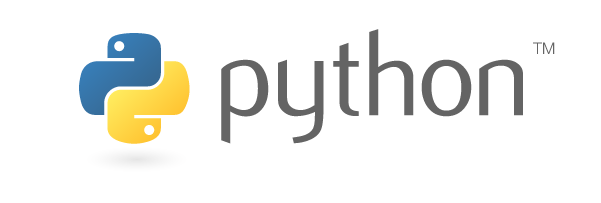
\includegraphics[width=180pt]{./pictures/python-logo-master-v3-TM.png}
      \caption[Python logo]{Python logo (source:
\href{https://www.python.org/static/community_logos/python-logo-master-v3-TM.png}{Python.org})}
      \label{fig:python}
  \end{figure}

Python is a high-level programming language that fully supports object-oriented and structured programming. Developed in the late 1980s, the first version 0.9.0 was released in 1991. In 2008, Python 3.0 was released. Currently, the most up-to-date version available is 3.6.\cite{diveintopython}

It was designed as a syntactically simple language, using whitespace intendantion instead of brackets and English words rather than punctuation. It is a dynamically-typed language, which means it is not neccessary to specify a data-type when defining a variable. For its simplicity and readability, Python is often considered a good first programming language to learn.

One of the key advantages of Python is its high extensibility. It provides large standard libraries and also an extensive number of other modules, packages and libraries, so most of the common programming tasks are already solved, scripted and made available.



\section{GitHub}

\begin{figure}[H] \centering
      
\includegraphics[width=170pt]{./pictures/github.png}
      \caption[GitHub logo]{GitHub logo (source:
\href{GitHub}{GitHub.com})}
      \label{fig:GitHub}
  \end{figure}

GitHub is a web-based Git repository hosting service with a graphical interface. Git is an open-source version control system for tracking changes in text files, typically used for source code management.\cite{git}  On top of the standard Git functionality, GitHub provides a number of its own features, including forking (copying a repository), pull requests, or bug tracking. GitHub also offers a desktop application.

\section{Geospatial Data Abstraction Library - GDAL/OGR}

\begin{figure}[H] \centering
      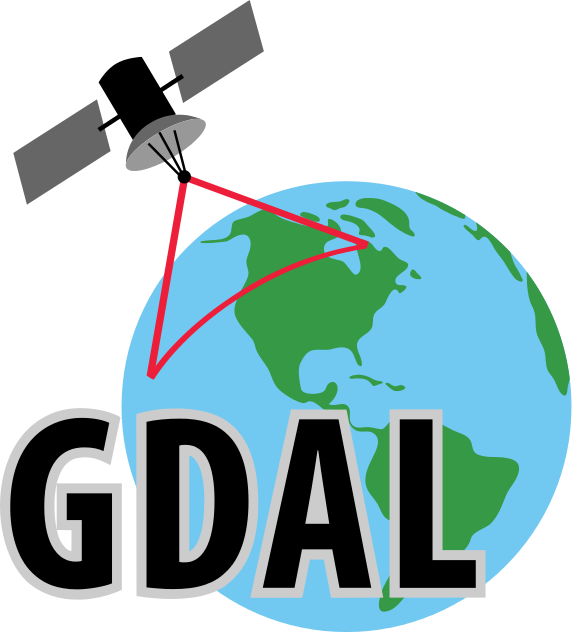
\includegraphics[width=130pt]{./pictures/gdal.png}
      \caption[GDAL logo]{GDAL logo (source:{\cite{gdal}})}
      \label{fig:GDAL}
  \end{figure}

Geospatial Data Abstraction Library (GDAL/OGR) is the most widely used geospatial data acces library for raster and vector geospatial data formats. It is released under an X/MIT style Open Source license by the Open Source Geospatial Foundation and it is written in C++ and C programming languages. As for operating systems, it can run under Linux, Solaris, Mac OS X and Microsoft Windows.\cite{gdal}

The first version was released by Frank Warmerdam in 2000 and the last stable version 2.2.3 was released in November 2017.\cite{gdalrelease}


The OGR library was developed separately but is now a part of the GDAL source tree. GDAL used to work with raster data and OGR with vector data. Starting with GDAL 2.0, however, the two have been integrated more tightly.

For its extensive capabilities and comprehensive set of functionalities, the GDAL/OGR library is widely used by both commercial and non-commercial GIS projects and programs. The list of software programs that uses it includes Google Earth, ArcGIS, GRASS GIS and many others.\cite{gdalogr} 
